\begin{frame}[fragile]

  \vspace{-10pt}

  {\Huge Thread safety and \\ atomic operations}

  \vspace{10pt}

  \textbf{Learning objectives:}
  \begin{itemize}
    \item{Understand that coordination techniques for low-count CPU threading are not scalable.}
    \item{Understand how atomics can parallelize the \textbf{scatter-add} pattern.}
    \item{Gain \textbf{performance intuition} for atomics on the CPU and GPU, for different data types and contention rates.}
    %\item{Understand a common thread-scalable \textbf{array-filling} algorithm.}
  \end{itemize}

  \vspace{-20pt}

\end{frame}

%==========================================================================

\begin{frame}[fragile]{Examples: Histogram}

 \begin{tikzpicture}[remember picture, overlay]
    \node [shift={(-6.4cm,1.10cm)}]  at (current page.south east)
      {%
      \begin{tikzpicture}[remember picture, overlay]
        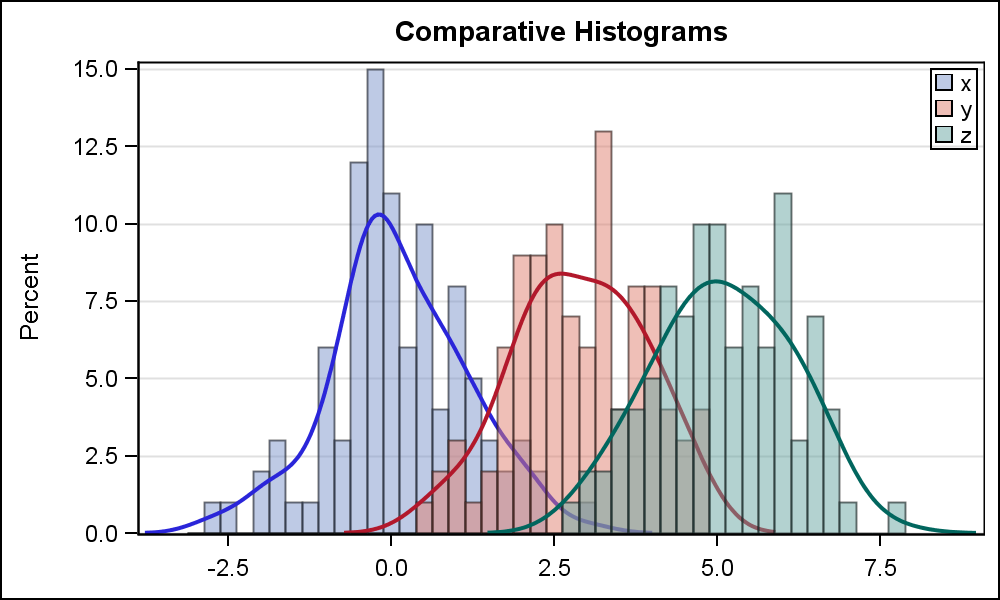
\includegraphics[width=0.50\textwidth]{figures/Histograma}
      \end{tikzpicture}
      };
  \end{tikzpicture}

  \begin{textblock*}{0.30\textwidth}(0.60\textwidth,0.91\textheight)
    \begin{tiny}
    http://www.farmaceuticas.com.br/tag/graficos/
    \end{tiny}
  \end{textblock*}

  \textbf{\ul{Histogram kernel:}}
  \begin{code}[linebackgroundcolor={
      },
      keywords={}, frame=single
    ]
parallel_for(N, KOKKOS_LAMBDA(const size_t index) {
    const Something value = ...;
    const size_t bucketIndex = computeBucketIndex(value);
    ++_histogram(bucketIndex);
  });
  \end{code}

  \pause

  {\color{red} \textbf{Problem}:} Multiple threads may try to write to the same location.

  \vspace{10pt}
  \pause

  \textbf{Solution strategies}:
  \begin{itemize}
    \item {Locks: not feasible on GPU}
    \item {Thread-private copies:\\ not thread-scalable}
    \item {Atomics}
  \end{itemize}

  \vspace{20pt}

\end{frame}

%==========================================================================

\begin{frame}[fragile]{Atomics}

  \ul{\textbf{Atomics}: the portable and thread-scalable solution}

  \begin{code}[linebackgroundcolor={
      },
      keywords={}, frame=single
    ]
parallel_for(N, KOKKOS_LAMBDA(const size_t index) {
    const Something value = ...;
    const int bucketIndex = computeBucketIndex(value);
    Kokkos::atomic_add(&_histogram(bucketIndex), 1);
  });
  \end{code}

  \pause
  \vspace{0pt}

  \begin{itemize}[<+->]
    \item {Atomics are the \textbf{only scalable} solution to thread safety.}
    \item {Locks are \textbf{not portable}.}
    \item {Data replication is \textbf{not thread scalable}.}
  \end{itemize}

  \vspace{0pt}

\end{frame}

%==========================================================================

\begin{frame}[fragile]{Performance of atomics (0)}

  \ul{\textbf{How expensive are atomics?}}

  \vspace{10pt}

  Thought experiment: scalar integration

  \begin{code}[linebackgroundcolor={
      },
      keywords={}
    ]
operator()(const unsigned int intervalIndex,
           double & valueToUpdate) const {
  double contribution = function(...);
  valueToUpdate += contribution;
}
  \end{code}

  \pause
  \vspace{10pt}
  Idea: what if we instead do this with \texttt{parallel\_for} and atomics?

  \begin{code}[linebackgroundcolor={
      },
      keywords={}
    ]
@grayoperator()(const unsigned int intervalIndex) const {
  const double contribution = function(...);@gray
  @boldKokkos::atomic_add@bold(&globalSum, contribution);
@gray}@gray
  \end{code}

  \vspace{0pt}
  How much of a performance penalty is incurred?

\end{frame}

%==========================================================================

\begin{frame}[fragile]{Performance of atomics (1)}

  \ul{\textbf{Two costs:}} (independent) {\color{blue}work} and {\color{darkred}coordination}.

  \vspace{-5pt}

  \begin{code}[linebackgroundcolor={
        \btLstHL<1->{4}{blue!20}
      },
      keywords={}
    ]
@warningparallel_reduce@warning(numberOfIntervals,
  KOKKOS_LAMBDA (const unsigned int intervalIndex,
                 double & valueToUpdate) {
    valueToUpdate += function(...);
  }, totalIntegral);
  \end{code}

  \vspace{10pt}
  \pause

  \ul{\textbf{Experimental setup}}

  \begin{code}[linebackgroundcolor={
      },
      frame=single,
      keywords={}
    ]
@grayoperator()(const unsigned int index) const {@gray
  Kokkos::atomic_add(&globalSums[index % atomicStride], 1);
@gray}@gray
  \end{code}

  \vspace{-5pt}

  \begin{itemize}
    \item{This is the most extreme case: {\color{darkred}all coordination} and {\color{darkred}no work}.}

    \item{Contention is captured by the \texttt{atomicStride}. \\
          \hspace{20pt}\texttt{atomicStride} $\rightarrow$ 1 \hspace{16pt}$\Rightarrow$ Scalar integration ({\color{darkred}bad}) \\
          \hspace{20pt}\texttt{atomicStride} $\rightarrow$ large $\Rightarrow$ Independent ({\color{darkgreen}good})
     }
  \end{itemize}

  \vspace{-15pt}

\end{frame}

%==========================================================================

\begin{frame}[fragile]{Performance of atomics (2)}

  \ul{\textbf{Atomics performance:} 1 million adds, \textbf{no} work per kernel}

  \vspace{0pt}

  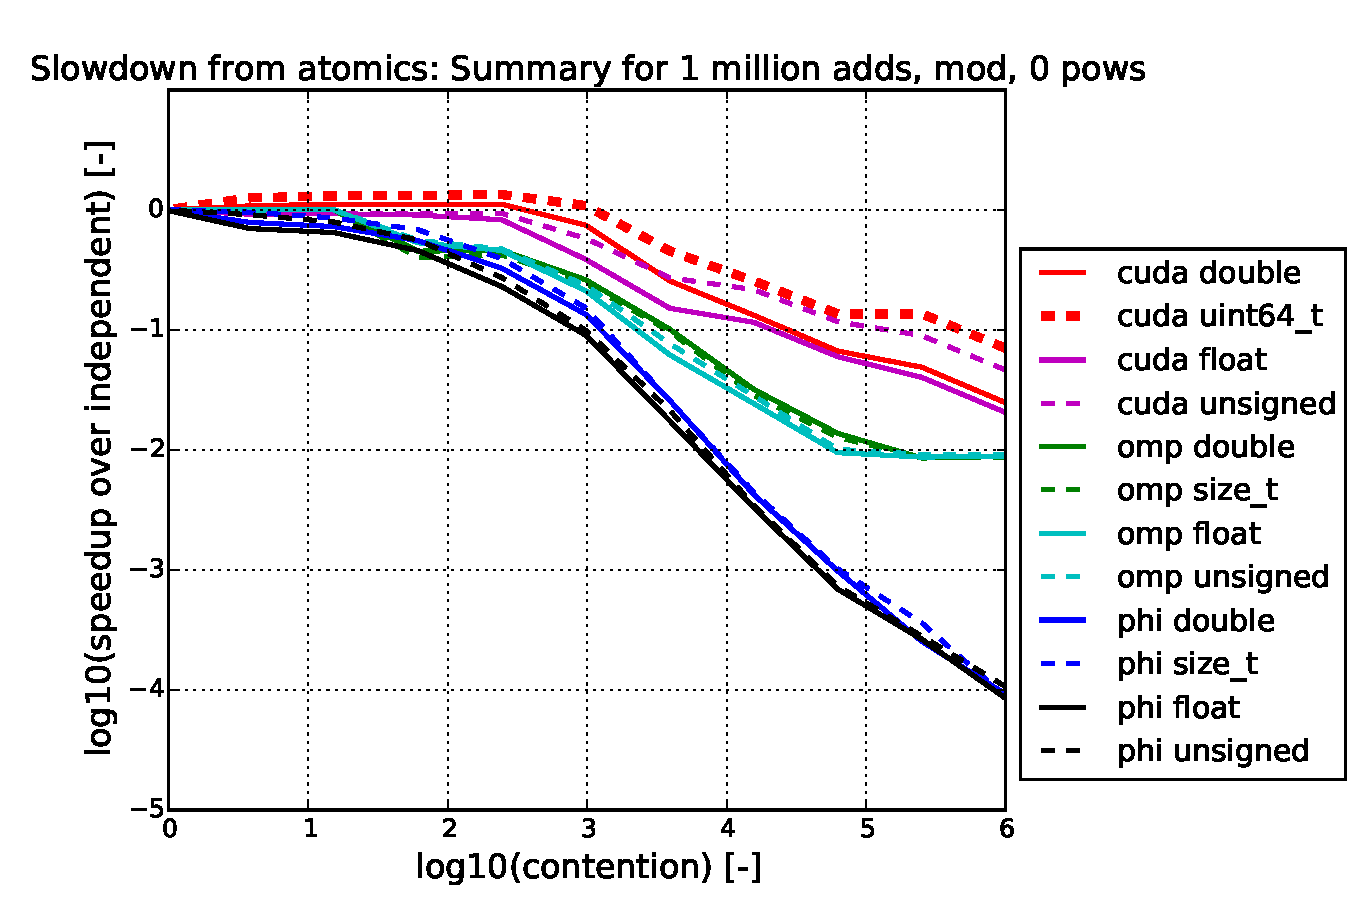
\includegraphics[width=1.00\textwidth]{figures/AtomicAddTest_slowdown_summary_mod_00pows.pdf}

  \begin{textblock*}{0.50\textwidth}(0.10\textwidth,0.45\textheight)
    \rotatebox{90}{Note: \textbf{log scale}}
  \end{textblock*}

  \pause

  \begin{textblock*}{0.70\textwidth}(0.23\textwidth,0.285\textheight)
    \only<2>{\textbf{Low(?) penalty for low contention}}
  \end{textblock*}

  \begin{tikzpicture}[remember picture, overlay]
    \node [shift={(2.40cm,6.05cm)}]  at (current page.south west)
      {%
      \begin{tikzpicture}[remember picture, overlay]
        \draw<2->[blue,ultra thick] (0.0,0.0) rectangle (2.00cm, 0.45cm);
      \end{tikzpicture}
      };
  \end{tikzpicture}


  \begin{textblock*}{0.70\textwidth}(0.35\textwidth,0.74\textheight)
    \only<2>{\textbf{High penalty for \\ high contention}}
  \end{textblock*}

  \begin{tikzpicture}[remember picture, overlay]
    \node [shift={(6.75cm,1.80cm)}]  at (current page.south west)
      {%
      \begin{tikzpicture}[remember picture, overlay]
        \draw<2->[red,ultra thick] (0.0,0.0) rectangle (2.25cm, 4.00cm);
      \end{tikzpicture}
      };
  \end{tikzpicture}
\end{frame}
\setcounter{subfigure}{0}% Reset subfigure counter

%==========================================================================

\begin{frame}[fragile]{Performance of atomics (3)}

  \ul{\textbf{Atomics performance:} 1 million adds, \textbf{some} work per kernel}

  \vspace{0pt}

  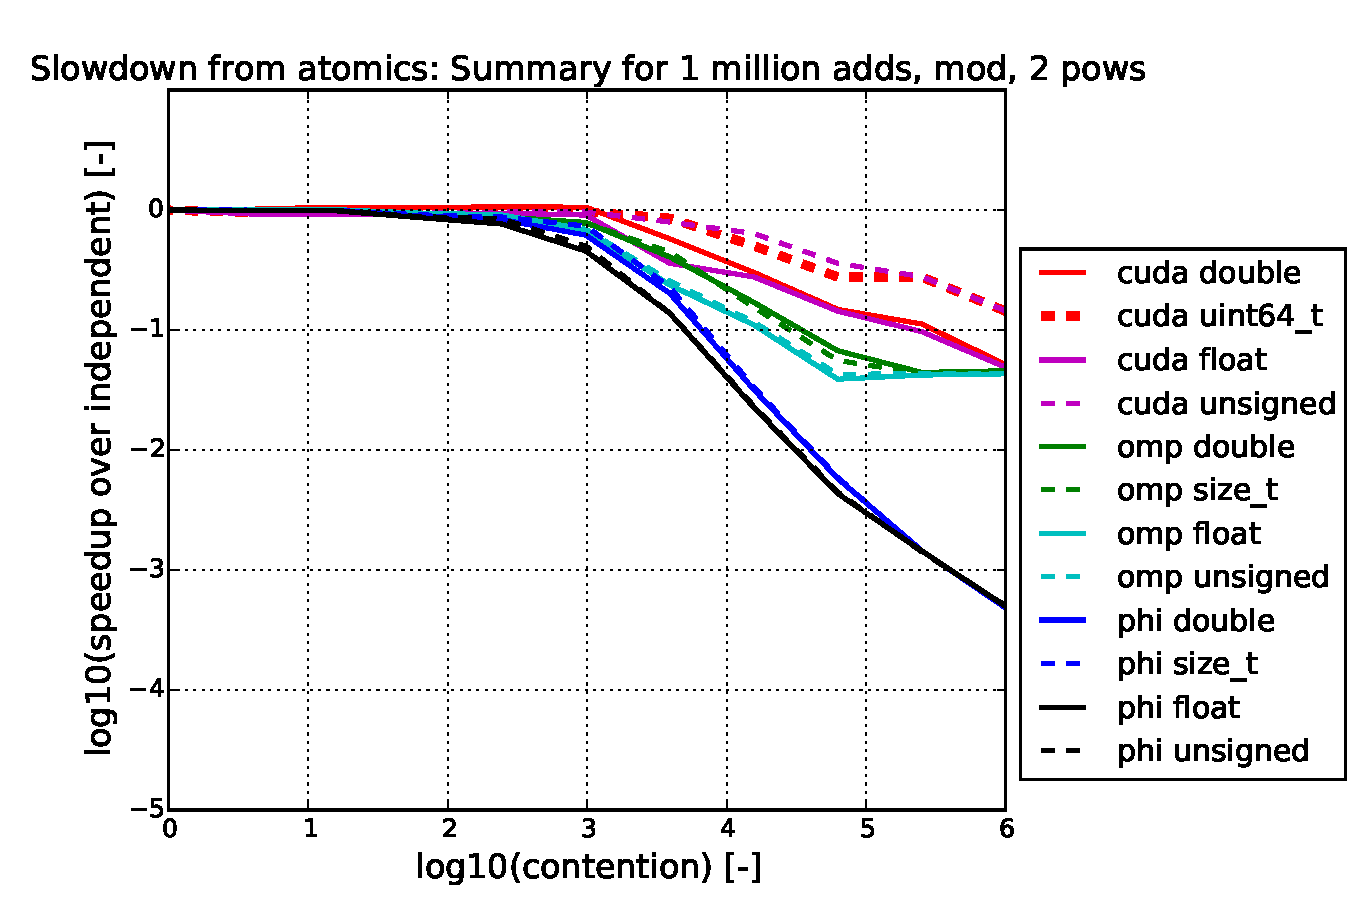
\includegraphics[width=1.00\textwidth]{figures/AtomicAddTest_slowdown_summary_mod_02pows.pdf}

  \begin{textblock*}{0.50\textwidth}(0.10\textwidth,0.45\textheight)
    \rotatebox{90}{Note: \textbf{log scale}}
  \end{textblock*}

  \begin{textblock*}{0.70\textwidth}(0.23\textwidth,0.285\textheight)
    \textbf{No penalty for low contention}
  \end{textblock*}

  \begin{tikzpicture}[remember picture, overlay]
    \node [shift={(2.40cm,5.90cm)}]  at (current page.south west)
      {%
      \begin{tikzpicture}[remember picture, overlay]
        \draw[blue,ultra thick] (0.0,0.0) rectangle (2.75cm, 0.52cm);
      \end{tikzpicture}
      };
  \end{tikzpicture}


  \begin{textblock*}{0.70\textwidth}(0.35\textwidth,0.74\textheight)
    \textbf{High penalty for \\ high contention}
  \end{textblock*}

  \begin{tikzpicture}[remember picture, overlay]
    \node [shift={(6.75cm,1.80cm)}]  at (current page.south west)
      {%
      \begin{tikzpicture}[remember picture, overlay]
        \draw[red,ultra thick] (0.0,0.0) rectangle (2.25cm, 4.00cm);
      \end{tikzpicture}
      };
  \end{tikzpicture}
\end{frame}
\setcounter{subfigure}{0}% Reset subfigure counter

%==========================================================================

\begin{frame}[fragile]{Performance of atomics (4)}

  \ul{\textbf{Atomics performance:} 1 million adds, \textbf{lots of} work per kernel}

  \vspace{0pt}

  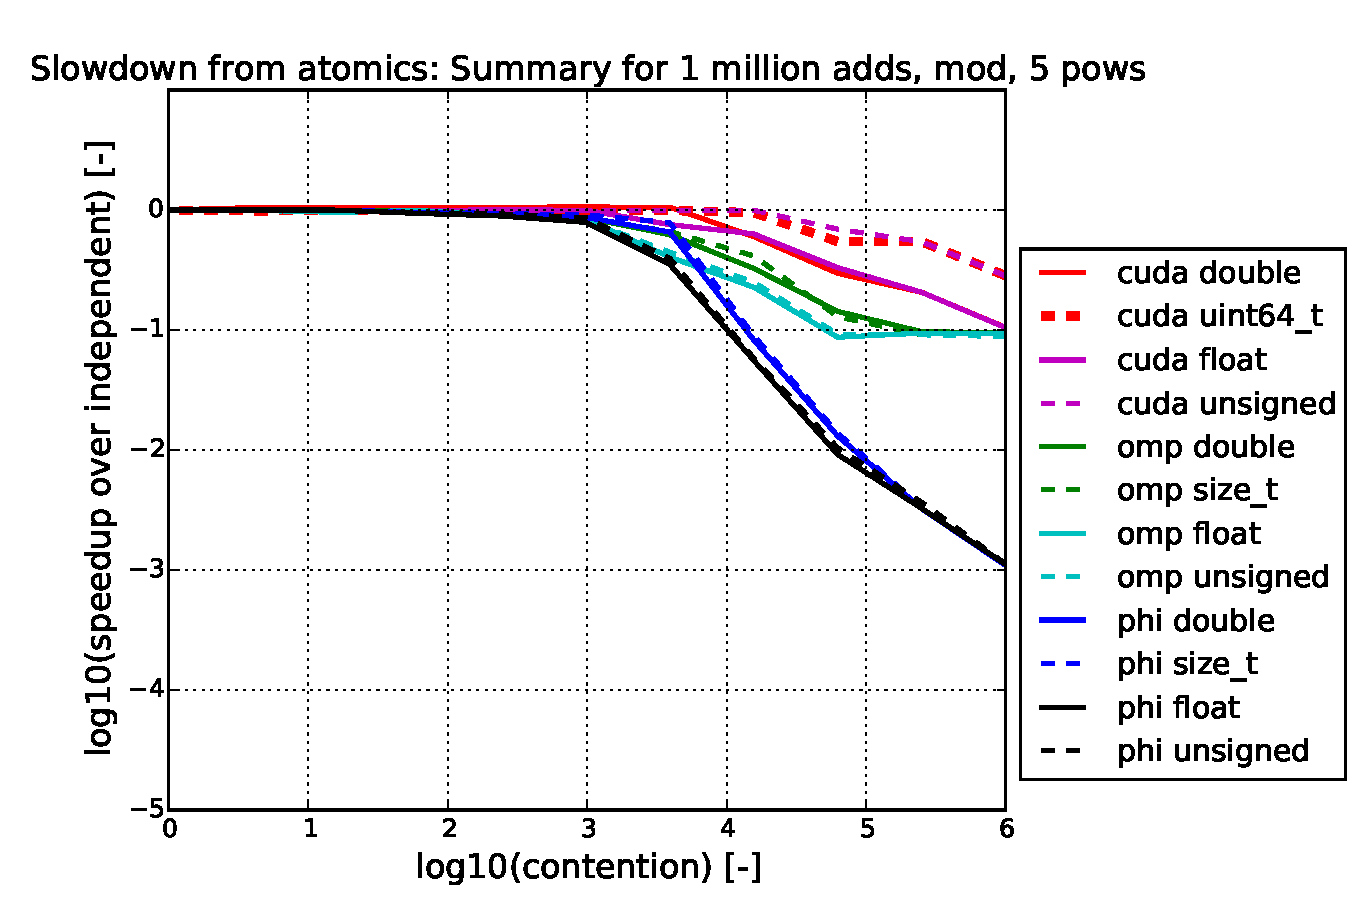
\includegraphics[width=1.00\textwidth]{figures/AtomicAddTest_slowdown_summary_mod_05pows.pdf}

  \begin{textblock*}{0.50\textwidth}(0.10\textwidth,0.45\textheight)
    \rotatebox{90}{Note: \textbf{log scale}}
  \end{textblock*}

  \begin{textblock*}{0.70\textwidth}(0.23\textwidth,0.285\textheight)
    \textbf{No penalty for low contention}
  \end{textblock*}

  \begin{tikzpicture}[remember picture, overlay]
    \node [shift={(2.40cm,5.90cm)}]  at (current page.south west)
      {%
      \begin{tikzpicture}[remember picture, overlay]
        \draw[blue,ultra thick] (0.0,0.0) rectangle (3.50cm, 0.52cm);
      \end{tikzpicture}
      };
  \end{tikzpicture}


  \begin{textblock*}{0.70\textwidth}(0.35\textwidth,0.74\textheight)
    \textbf{High penalty for \\ high contention}
  \end{textblock*}

  \begin{tikzpicture}[remember picture, overlay]
    \node [shift={(6.75cm,1.80cm)}]  at (current page.south west)
      {%
      \begin{tikzpicture}[remember picture, overlay]
        \draw[red,ultra thick] (0.0,0.0) rectangle (2.25cm, 4.00cm);
      \end{tikzpicture}
      };
  \end{tikzpicture}
\end{frame}
\setcounter{subfigure}{0}% Reset subfigure counter

%==========================================================================

\begin{frame}[fragile]{Advanced features}

\textbf{\ul{Atomics on arbitrary types}:}

\begin{itemize}
\item Atomic operations work if the corresponding operator exists,
  \hspace{50pt}i.e., \texttt{atomic\_add} works on any data type with ``+''.
\item {Atomic exchange works on any data type.}
\end{itemize}
\vspace{-10pt}
  \begin{code}[linebackgroundcolor={
      },
      keywords={}
    ]
// Assign *dest to val, return former value of *dest
template<typename T>
T atomic_exchange(T * dest, T val);
// If *dest == comp then assign *dest to val
// Return true if succeeds.
template<typename T>
bool atomic_compare_exchange_strong(T * dest, T comp, T val);
\end{code}

\end{frame}

%==========================================================================

\begin{frame}[fragile]{Memory traits}

  \textbf{\ul{Slight detour: \texttt{View} memory traits}:}

  \begin{itemize}
    \item Beyond a \texttt{Layout} and \texttt{Space}, \texttt{Views} can have memory traits.
    \item Memory traits either provide \textbf{convenience} or allow for certain \textbf{hardware-specific optimizations} to be performed.
  \end{itemize}

  Example: If all accesses to a \texttt{View} will be atomic, use the \texttt{Atomic} memory trait:

  \vspace{-2pt}
  \begin{code}[keywords={}]
    View<double**, Layout, Space,
         @boldMemoryTraits<Atomic> @bold> forces(...);
  \end{code}

  \vspace{5pt}
  \pause

  Many memory traits exist or are experimental, including \texttt{Atomic}, \texttt{Unmanaged}, \texttt{Restrict}, and \texttt{RandomAccess}.

  \vspace{-15pt}

\end{frame}

%==========================================================================

\begin{frame}[fragile]{RandomAccess memory trait}

  \textbf{\ul{Example: \texttt{RandomAccess} memory trait}:}

  \vspace{3pt}

  On \textbf{GPUs}, there is a special pathway for fast \textbf{read-only}, \textbf{random} access, originally designed for textures.

  \vspace{5pt}
  \pause

  In the early days you had to access this via \textbf{CUDA}:
  \vspace{5pt}
  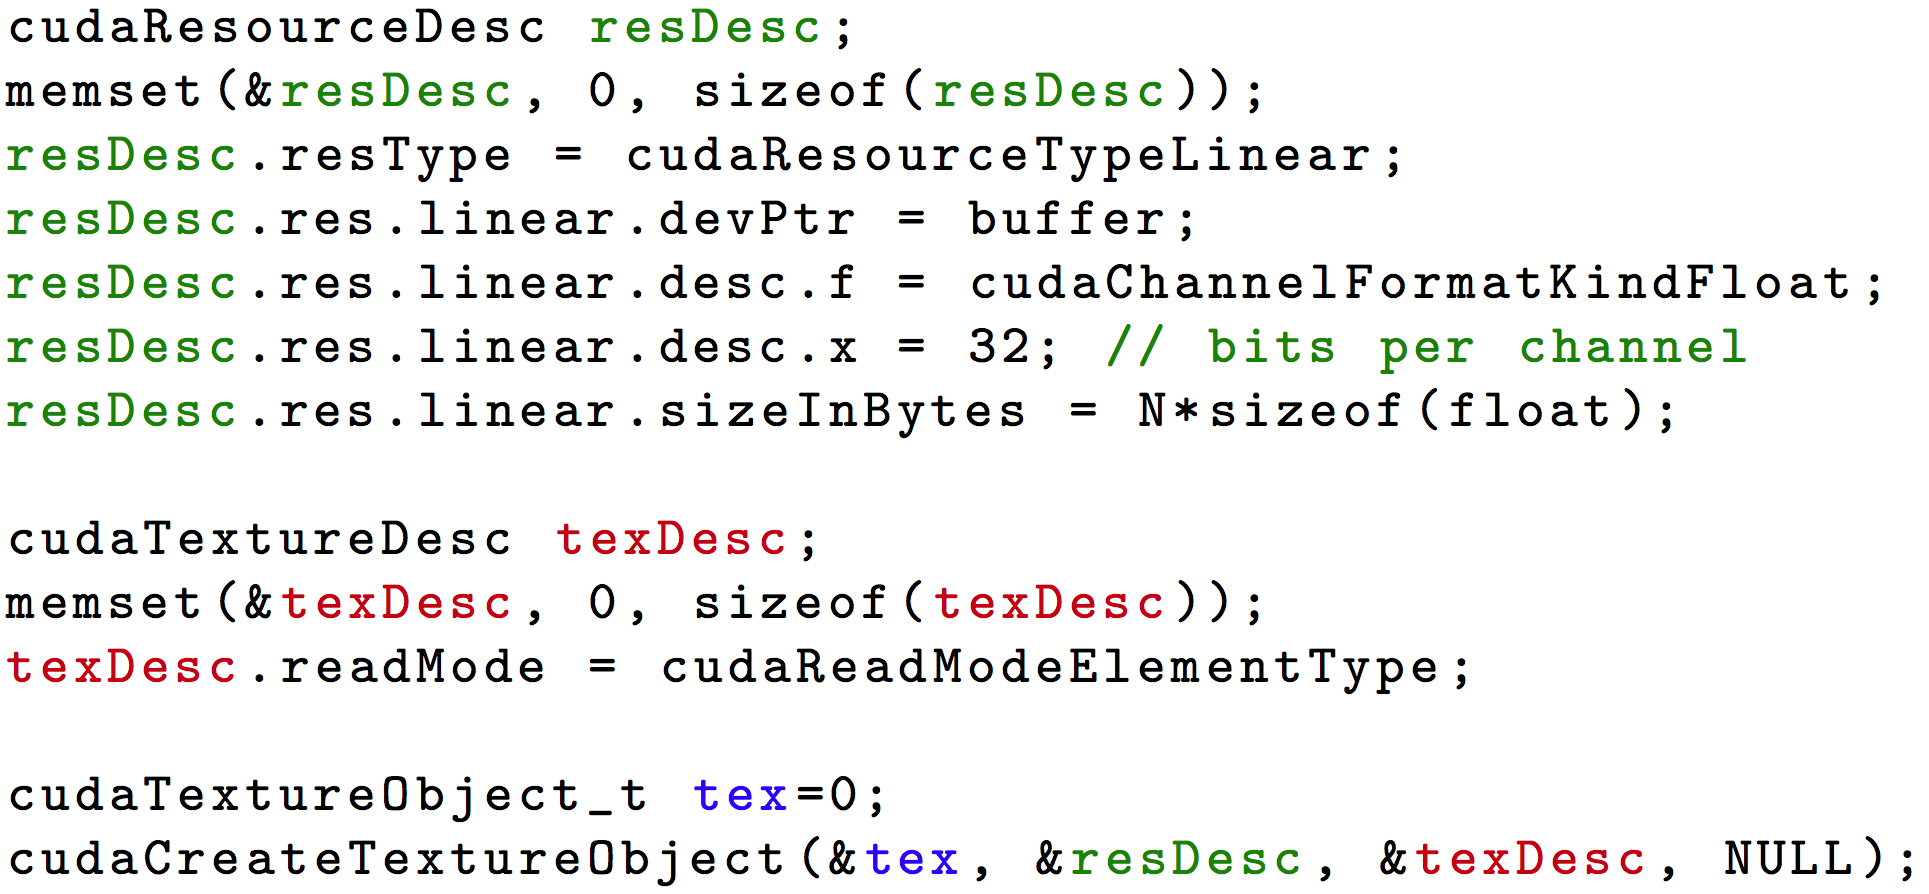
\includegraphics[width=0.80\textwidth]{figures/CudaTextureCode}

  \vspace{0pt}
  \pause
  \textbf{Kokkos} can hide mechanisms like that as simple as:
  \vspace{-5pt}

  \begin{code}[keywords={}]
View< @boldconst@bold double***, Layout, Space,
     @boldMemoryTraits<RandomAccess> @bold> name(...);
  \end{code}

\end{frame}

%==========================================================================

\begin{frame}[fragile]{Scatter Contribute (1)}

  Histogram generation is an example of the \textbf{Scatter Contribute} pattern.
 
  \begin{itemize}
    \item{Like a reduction but with many results.}
    \item{Number of results scales with number of inputs.}
    \item{Each results gets contributions from a small number of inputs/iterations.}
    \item{Uses an inputs-to-results map not inverse.}
  \end{itemize}

  \textbf{Examples:}
  \begin{itemize}
    \item{Particles contributing to neighbors forces.}
    \item{Cells contributing forces to nodes.}
    \item{Computing histograms.}
    \item{Computing a density grid from point source contributions.}
  \end{itemize}

\end{frame}

\begin{frame}[fragile]{Scatter Contribute (2)}

  \textbf{Compute forces on particles via neighbor contributions}

  This kernel uses Newtons Third Law: Actio = Reactio
  \begin{code}[keywords={void,int,parallel_for,for,View}]
void compute_forces(View<real3*> x, View<real3*> f,
	            View<int**> neighs, Interaction force) {
  int N = x.extent(0);
  int num_neighs = neighs.extent(1);
  parallel_for("ForceCompute", N, KOKKOS_LAMBDA(int i) {
    for(int j=0; j<num_neighs; j++) {
      real3 df = force.compute(x(i),x(neighs(i,j)));
      f(i) += df;
      f(j) -= df;
    }
  });
}
  \end{code}

  \pause
  \textbf{This kernel has a race condition on \texttt{f} though!}

\end{frame}

\begin{frame}[fragile]{ScatterView (0)}

  There are two useful algorithms:.
 
  \begin{itemize}
	  \item{\textbf{Atomics:} thread-scalable but depends on atomic performance.}
	  \item{\textbf{Data Replication:} every thread owns a copy of the output, not thread-scalable but good for low ($<16$) threads count architectures.}
  \end{itemize}

  \pause
  \begin{block}{Important Capability: ScatterView}
	  ScatterView can transparently switch between \textbf{Atomic} and \textbf{Data Replication} based scatter algorithms.
  \end{block}
  \pause
 	
  \begin{itemize}
	  \item{Abstracts over scatter contribute algorithms.}
	  \item{Compile time choice with backend-specific defaults.}
          \item{Only limited number of operations are supported.}
	  \item{Part of Kokkos Containers (in Kokkos 3.2 still experimental).}
  \end{itemize}

\end{frame}


\begin{frame}[fragile]{ScatterView (1)}
\textbf{Creating a ScatterView:}

Usually a \texttt{ScatterView} wraps an existing \texttt{View}
\pause
\begin{itemize}
  \item Allows the \textbf{atomic} variant to work without extra allocation.
\end{itemize}
\pause
\begin{code}[keywords={void,ScatterView,View,int}]
void compute_forces(View<real3*> x, View<real3*> f, 
	            View<int**> neighs, Interaction force) {
Kokkos::Experimental::ScatterView<real3*> scatter_f(f);
...
\end{code}

\pause
\textbf{Accessing the \texttt{ScatterView}}

In the kernel obtain an atomic or thread-local accessor.

  \begin{code}[keywords={access,auto,for,int}]
parallel_for("ForceCompute", N, KOKKOS_LAMBDA(int i) {
  auto f_a = scatter_f.access();
  for(int j=0; j<num_neighs; j++) {
    real3 df = force.compute(x(i),x(neighs(i,j)));
    f_a(i) += df;
    f_a(j) -= df;
  }
});
  \end{code}

  \pause
	\textbf{Only the \texttt{+=} and \texttt{-=} operators are available!}
\end{frame}

\begin{frame}[fragile]{ScatterView (2)}
We are missing one step though:
\pause
\textbf{Contribute back to the original view.}

  \begin{code}[keywords={void,View,ScatterView,int,contribute}]
void compute_forces(View<real3*> x, View<real3*> f,
	            View<int**> neighs, Interaction force) {
  Kokkos::Experimental::ScatterView<real3*> scatter_f(f);
  parallel_for("ForceCompute", N, KOKKOS_LAMBDA(int i) {
    ...
  });
  Kokkos::Experimental::contribute(f,scatter_f);
  \end{code}
\pause
\begin{itemize}
	\item No-op when \texttt{scatter\_f} uses \textbf{atomic} access
	\item Combines thread-local arrays in case of data duplication
\end{itemize}

\pause
	\begin{block}{Important Point}
		Reuse ScatterView if possible: creating and destroying data duplicates is costly and should be avoided
	\end{block}
\end{frame}

\begin{frame}[fragile]{ScatterView (3)}
	When reusing a \texttt{ScatterView} the duplicates have to be reset.

\begin{code}[keywords={reset}]
scatter_f.reset();
\end{code}

\pause
\textbf{The complete picture:}

  \begin{code}[keywords={ScatterView,reset,access,contribute}]
void compute_forces(View<real3*> x, View<real3*> f,
                    ScatterView<real3*> scatter_f,
	            View<int**> neighs, Interaction force) {
  scatter_f.reset();
  int N = x.extent(0);
  int num_neighs = neighs.extent(1);
  parallel_for("ForceCompute", N, KOKKOS_LAMBDA(int i) {
    auto f_a = scatter_f.access();
    for(int j=0; j<num_neighs; j++) {
      real3 df = force.compute(x(i),x(neighs(i,j)));
      f_a(i) += df;
      f_a(j) -= df;
    }
  });
  Kokkos::Experimental::contribute(f,scatter_f);
}
  \end{code}	
\end{frame}


\begin{frame}[fragile]{ScatterView (4)}
\textbf{But I need something else than a Sum!}

\pause
\texttt{ScatterView} has more options including the reduction op.

\begin{code}[keywords={template,class}]
  template<class DataType, class Layout, class Space,
	   class Operation, int Duplication, int Contribution>
  class ScatterView;
\end{code}
	\begin{itemize}
		\item \texttt{DataType}, \texttt{Layout}, \texttt{Space}:  as in \texttt{Kokkos::View}
		\item \texttt{Operation}: \texttt{ScatterSum}, \texttt{ScatterProd}, \texttt{ScatterMin}, or \texttt{ScatterMax}.
		\item \texttt{Duplication}: Whether to duplicate values per thread.
		\item \texttt{Contribution}: Whether to use \textbf{atomics}.
	\end{itemize}

\end{frame}


\begin{frame}[fragile]{Exercise ScatterView}

  \begin{small}
  \begin{itemize}
  \item Location: \ExerciseDirectory{scatter\_view/Begin}
  \item Assignment: Convert scatter\_view\_loop to use \texttt{ScatterView}.
  \item Compile and run on both CPU and GPU
  \end{itemize}
  \end{small}

\begin{code}
  # Compile for CPU
  cmake -B build_openmp -DKokkos_ENABLE_OPENMP=ON
  cmake --build build_openmp
  # Run on CPU
  ./build_openmp/scatterview -S 26
  # Note the warnings, set appropriate environment variables
  # Compile for GPU
  cmake -B build_cuda -DKokkos_ENABLE_CUDA=ON
  cmake --build build_cuda
  # Run on GPU
  ./build_cuda/scatterview -S 26
\end{code}

  \begin{scriptsize}
  \begin{itemize}
  \item Compare performance on CPU of the three variants
  \item Compare performance on GPU of the two variants
  \item Vary problem size: first and second optional argument
  \end{itemize}
  \end{scriptsize}

\end{frame}
%==========================================================================

\begin{frame}{Section Summary}

  \begin{itemize}
    \item Atomics are the only thread-scalable solution to thread safety.
      \begin{itemize}
        \item Locks or data replication are \textbf{not portable or scalable}
      \end{itemize}
    \item Atomic performance \textbf{depends on ratio} of independent work and atomic operations.
      \begin{itemize}
        \item With more work, there is a lower performance penalty, because of increased opportunity to interleave work and atomic.
      \end{itemize}
    \item The \texttt{Atomic} \textbf{memory trait} can be used to make all accesses to a view atomic.
    \item The cost of atomics can be negligible:
      \begin{itemize}
        \item \textbf{CPU} ideal: contiguous access, integer types
        \item \textbf{GPU} ideal: scattered access, 32-bit types
      \end{itemize}
    \item Many programs with the \textbf{scatter-add} pattern can be thread-scalably parallelized using atomics without much modification.
    %\item{Scatter-atomic-add \emph{can} have \textbf{negligible} cost for low contention ($< \sim100$) and non-trivial work.}
  \end{itemize}

\end{frame}
